% =============================================================================
% Dual-Model Aerial Image Understanding Pipeline - Project Report
% -----------------------------------------------------------------------------
% Build:
%   cd docs && pdflatex -interaction=nonstopmode report.tex
% (run twice so cross-references resolve)
%
% Dependencies: standard TeX Live (article, tikz, booktabs, listings, hyperref,
% xcolor, graphicx, amsmath, caption, subcaption, geometry, float, enumitem).
% =============================================================================

\documentclass[11pt,a4paper]{article}

\usepackage[margin=2.3cm]{geometry}
\usepackage[utf8]{inputenc}
\usepackage[T1]{fontenc}
\usepackage{lmodern}
\usepackage{microtype}
\usepackage{graphicx}
\usepackage{float}
\usepackage{caption}
\usepackage{subcaption}
\usepackage{booktabs}
\usepackage{array}
\usepackage{tabularx}
\usepackage{xcolor}
\usepackage{enumitem}
\usepackage{amsmath, amssymb}
\usepackage{listings}
\usepackage{tikz}
\usetikzlibrary{shapes.geometric, arrows.meta, positioning, fit, calc, backgrounds, decorations.pathreplacing}
\usepackage[hidelinks, colorlinks=true, linkcolor=teal, urlcolor=teal, citecolor=teal]{hyperref}

% -----------------------------------------------------------------------------
% Colors and listing styles
% -----------------------------------------------------------------------------
\definecolor{codebg}{RGB}{248,248,248}
\definecolor{codekw}{RGB}{0,85,153}
\definecolor{codestr}{RGB}{170,55,55}
\definecolor{codecom}{RGB}{95,120,95}
\definecolor{codeln}{RGB}{150,150,150}
\definecolor{accent}{RGB}{0,110,130}

\lstdefinestyle{commonstyle}{
    backgroundcolor=\color{codebg},
    basicstyle=\ttfamily\small,
    breaklines=true,
    keywordstyle=\color{codekw}\bfseries,
    stringstyle=\color{codestr},
    commentstyle=\color{codecom}\itshape,
    numberstyle=\tiny\color{codeln},
    numbers=left,
    numbersep=7pt,
    frame=single,
    rulecolor=\color{black!15},
    tabsize=2,
    showstringspaces=false,
    captionpos=b,
    xleftmargin=1.3em,
    framexleftmargin=1em,
}
\lstdefinelanguage{yaml}{
    keywords={true,false,null,yes,no},
    keywordstyle=\color{codekw}\bfseries,
    sensitive=false,
    comment=[l]{\#},
    morestring=[b]',
    morestring=[b]",
}
\lstdefinestyle{yaml}{style=commonstyle, language=yaml}
\lstdefinestyle{python}{style=commonstyle, language=Python}
\lstdefinestyle{bash}{style=commonstyle, language=bash}

% -----------------------------------------------------------------------------
% TikZ styles
% -----------------------------------------------------------------------------
\tikzset{
  block/.style      = {rectangle, rounded corners=2pt, draw=black!60, fill=blue!5,
                       minimum height=9mm, minimum width=22mm, align=center,
                       font=\footnotesize},
  data/.style       = {rectangle, draw=black!60, fill=orange!10,
                       minimum height=9mm, minimum width=22mm, align=center,
                       font=\footnotesize},
  model/.style      = {rectangle, rounded corners=4pt, draw=black!70, thick,
                       fill=teal!10, minimum height=11mm, minimum width=26mm,
                       align=center, font=\footnotesize\bfseries},
  output/.style     = {rectangle, draw=black!60, fill=green!8,
                       minimum height=9mm, minimum width=22mm, align=center,
                       font=\footnotesize},
  arrow/.style      = {-{Stealth[length=2mm]}, thick, black!70},
  dashedarrow/.style= {-{Stealth[length=2mm]}, thick, dashed, black!60},
  grouplabel/.style = {font=\small\itshape, text=black!60},
}

% -----------------------------------------------------------------------------
% Title & metadata
% -----------------------------------------------------------------------------
\title{%
  \vspace{-1.2cm}
  \Large\textbf{A Dual-Model Deep Learning Pipeline for Aerial Image Understanding} \\[0.35em]
  \normalsize YOLOv8 Oriented Bounding-Box Detection $+$ U-Net Semantic Segmentation \\[-0.25em]
  \normalsize on AMD ROCm (Radeon RX 6700S)
}
\author{Aerial Image Segmentation Project}
\date{\today}

\begin{document}
\maketitle

\vspace{-1.2em}
\begin{abstract}
\noindent
This report describes a dual-model deep learning pipeline that combines two complementary
computer vision tasks---semantic segmentation and oriented object detection---to
produce a rich, pixel-accurate interpretation of aerial imagery. The system
trains two architecturally distinct networks independently: a U-Net on the ISPRS Potsdam
dataset for six-class pixel labelling, and a YOLOv8 model with an oriented
bounding-box (OBB) head on the VSAI vehicle dataset for rotation-aware object
localization. At inference time, the two models' outputs are fused geometrically
into a single composite visualization. The entire pipeline targets consumer-grade
AMD hardware (Radeon RX 6700S, RDNA2 mobile) via the ROCm software stack, with
Docker-based reproducibility and automated dataset acquisition. We document the
architecture, datasets, training methodology, inference fusion, testing strategy,
and the technical workarounds required for ROCm on unsupported mobile silicon.
\end{abstract}

\vspace{0.5em}
\tableofcontents
\vspace{0.5em}
\hrule
\vspace{1em}

% =============================================================================
\section{Introduction}
% =============================================================================

Aerial imagery analysis is a canonical multi-task computer vision problem. A single
overhead photograph typically contains both \emph{stuff} classes (road, vegetation,
rooftops, water) that are best described by dense per-pixel labels, and \emph{things}
(individual vehicles, buildings, aircraft) that are best localized by discrete
bounding boxes. Neither task alone produces a complete scene description: a semantic
segmentation network cannot count cars, and a detector cannot paint the road they
are parked on.

The approach presented here accepts that these are fundamentally different problems,
trains a specialist network for each, and fuses their outputs only at inference time.
This choice reflects three practical constraints:

\begin{enumerate}[leftmargin=*, itemsep=3pt]
  \item \textbf{Dataset asymmetry.} The best freely available datasets for the two
    tasks are annotated in incompatible ways. ISPRS Potsdam provides dense RGB masks
    with a six-class palette; VSAI provides oriented bounding boxes for two vehicle
    classes. No single dataset covers both annotation styles at scale.
  \item \textbf{Architectural specialization.} Semantic segmentation benefits from
    symmetric encoder-decoder networks with dense skip connections (e.g. U-Net);
    oriented-box detection benefits from anchor-free detection heads with angle
    regression (e.g. YOLOv8-OBB). A joint model would compromise both.
  \item \textbf{Hardware budget.} Training on an 80\,W mobile GPU requires keeping
    per-step compute small. Independent models can be trained sequentially with
    moderate batch sizes; a single multi-task model with a shared backbone would
    increase VRAM pressure non-trivially.
\end{enumerate}

\section{System Overview}

Figure~\ref{fig:pipeline} shows the end-to-end pipeline. The two
training tracks are fully decoupled: each has its own dataset, preprocessing,
loss function, optimizer, and schedule. Only at inference does a single RGB image
traverse both networks, with their outputs composed into a shared visualization.

\begin{figure}[H]
\centering
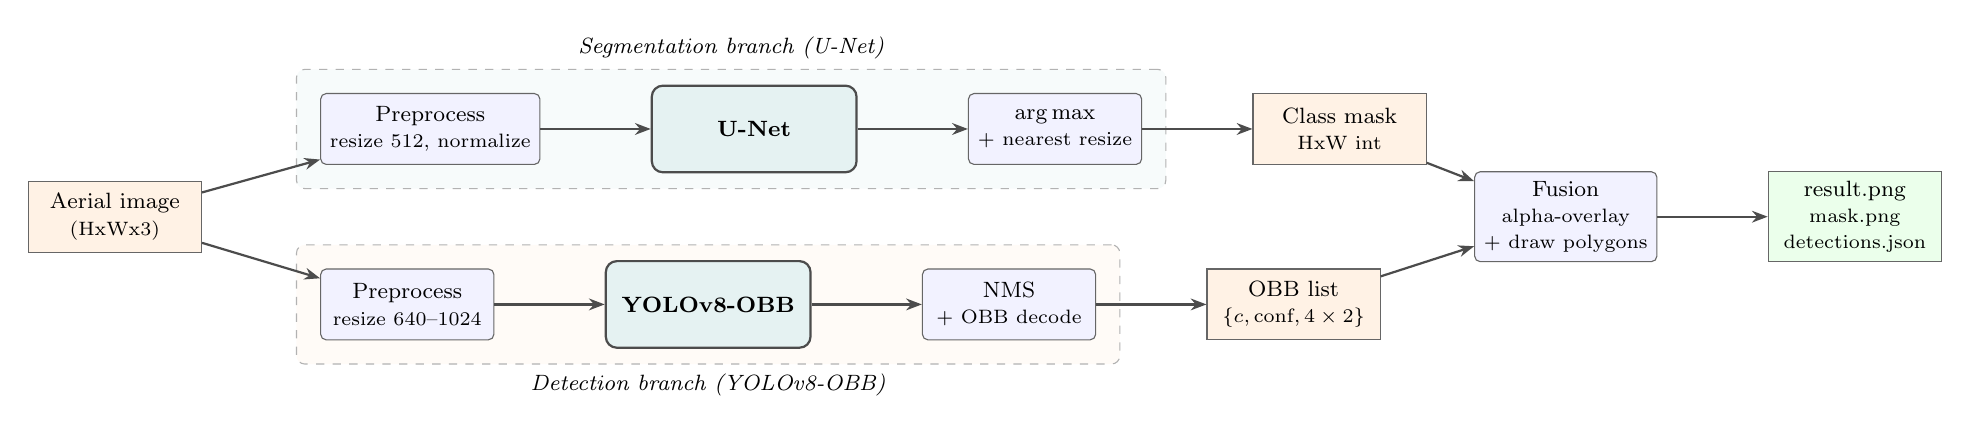
\begin{tikzpicture}[node distance=12mm and 14mm]

  \node[data] (img)    {Aerial image\\\scriptsize (HxWx3)};

  \node[block, above right=2mm and 15mm of img] (prep_unet) {Preprocess\\\scriptsize resize 512, normalize};
  \node[block, below right=2mm and 15mm of img] (prep_yolo) {Preprocess\\\scriptsize resize 640--1024};

  \node[model, right=of prep_unet] (unet) {U-Net};
  \node[model, right=of prep_yolo] (yolo) {YOLOv8-OBB};

  \node[block, right=of unet] (post_unet) {$\arg\max$\\\scriptsize + nearest resize};
  \node[block, right=of yolo] (post_yolo) {NMS\\\scriptsize + OBB decode};

  \node[data, right=of post_unet] (mask) {Class mask\\\scriptsize HxW int};
  \node[data, right=of post_yolo] (dets) {OBB list\\\scriptsize $\{c,\text{conf},4\times2\}$};

  \node[block, right=20mm of $(mask)!0.5!(dets)$] (fuse) {Fusion\\\scriptsize alpha-overlay\\\scriptsize + draw polygons};
  \node[output, right=of fuse] (out) {result.png\\\scriptsize mask.png\\\scriptsize detections.json};

  \draw[arrow] (img) -- (prep_unet);
  \draw[arrow] (img) -- (prep_yolo);
  \draw[arrow] (prep_unet) -- (unet);
  \draw[arrow] (prep_yolo) -- (yolo);
  \draw[arrow] (unet)      -- (post_unet);
  \draw[arrow] (yolo)      -- (post_yolo);
  \draw[arrow] (post_unet) -- (mask);
  \draw[arrow] (post_yolo) -- (dets);
  \draw[arrow] (mask) -- (fuse);
  \draw[arrow] (dets) -- (fuse);
  \draw[arrow] (fuse) -- (out);

  \begin{scope}[on background layer]
    \node[draw=black!30, dashed, rounded corners=3pt, fit=(prep_unet)(post_unet),
          inner sep=3mm, fill=teal!3, label=above:{\footnotesize\itshape Segmentation branch (U-Net)}] {};
    \node[draw=black!30, dashed, rounded corners=3pt, fit=(prep_yolo)(post_yolo),
          inner sep=3mm, fill=orange!3, label=below:{\footnotesize\itshape Detection branch (YOLOv8-OBB)}] {};
  \end{scope}
\end{tikzpicture}
\caption{The dual-model inference pipeline. The two branches are architecturally
and statistically independent; fusion is purely geometric.}
\label{fig:pipeline}
\end{figure}

\paragraph{Project layout.} The repository is organized around this separation:

\begin{center}\footnotesize
\begin{tabular}{ll}
\toprule
\texttt{data/}      & dataset download and PyTorch dataset classes \\
\texttt{models/}    & model definitions (U-Net, YOLO wrapper) \\
\texttt{train/}     & training entry points (\texttt{train\_unet.py}, \texttt{train\_yolo.py}) \\
\texttt{inference/} & fusion pipeline, visualization helpers \\
\texttt{utils/}     & shared utilities (config loader, device select, HSA override, seed, checkpointing) \\
\texttt{tests/}     & unit, integration, and ROCm hardware validation suites \\
\texttt{config.yaml} & single source of truth for all hyperparameters \\
\bottomrule
\end{tabular}
\end{center}

% =============================================================================
\section{Datasets}
% =============================================================================

Two public datasets, downloaded on first run via the \texttt{kagglehub} API, drive
the two training tasks.

\subsection{ISPRS Potsdam (U-Net)}

\begin{tabularx}{\linewidth}{l X}
\toprule
\textbf{Source}       & Kaggle: \texttt{deasadiqbal/private-data-1} (derived patches) \\
\textbf{Modality}     & Aerial orthophotos of Potsdam, Germany \\
\textbf{Images}       & 2\,400 pre-extracted patches (512$\times$512, TIFF) \\
\textbf{Annotation}   & RGB semantic masks, palette-encoded per pixel \\
\textbf{Classes}      & 6 \\
\textbf{Train/val}    & 80/20 random split (seed 42) \\
\bottomrule
\end{tabularx}

\begin{table}[H]
\centering
\footnotesize
\caption{Potsdam six-class RGB palette used by \texttt{PotsdamDataset}. Any pixel
color not in this table is mapped to class 5 (\emph{clutter}) as a safety fallback.}
\label{tab:potsdam-classes}
\begin{tabular}{clcccl}
\toprule
ID & Name & R & G & B & Swatch \\
\midrule
0 & impervious\_surface & 255 & 255 & 255 & \fcolorbox{black!40}{white}{\phantom{XX}} \\
1 & building            &   0 &   0 & 255 & \fcolorbox{black!40}{blue}{\phantom{XX}}  \\
2 & low\_vegetation     &   0 & 255 & 255 & \fcolorbox{black!40}{cyan}{\phantom{XX}}  \\
3 & tree                &   0 & 255 &   0 & \fcolorbox{black!40}{green}{\phantom{XX}} \\
4 & car                 & 255 & 255 &   0 & \fcolorbox{black!40}{yellow}{\phantom{XX}}\\
5 & clutter             & 255 &   0 &   0 & \fcolorbox{black!40}{red}{\phantom{XX}}   \\
\bottomrule
\end{tabular}
\end{table}

\subsection{VSAI OBB Vehicle Dataset (YOLO)}

\begin{tabularx}{\linewidth}{l X}
\toprule
\textbf{Source}       & Kaggle: \texttt{redzapdos123/vsai-dataset-yolo11-obb-format} \\
\textbf{Modality}     & Drone-captured vehicle patches \\
\textbf{Images}       & $\approx$1\,075 train / 537 val / 268 test (PNG, 1024$\times$1024) \\
\textbf{Annotation}   & YOLOv8 oriented-bounding-box format: \\
                      & \hspace{1em}\texttt{class\_id $x_1\,y_1\,x_2\,y_2\,x_3\,y_3\,x_4\,y_4$} (normalized corners) \\
\textbf{Classes}      & 2: \{small-vehicle, large-vehicle\} \\
\textbf{Split source} & Pre-defined by dataset publisher (\texttt{data.yaml} shipped inside archive) \\
\bottomrule
\end{tabularx}

\paragraph{Dynamic dataset-YAML generation.} VSAI ships with a \texttt{data.yaml}
that uses relative paths assuming a specific mount point. Because \texttt{kagglehub}
caches datasets at host-specific absolute paths, \texttt{data/download\_vsai.py}
re-emits a fresh \texttt{data/vsai\_dataset.yaml} on every invocation with an
absolute \texttt{path:} field and the original class names preserved. This keeps
training portable across hosts and containers without editing the bundled YAML.

% =============================================================================
\section{Model Architectures}
% =============================================================================

\subsection{U-Net for Semantic Segmentation}

U-Net~\cite{ronneberger2015unet} is a fully-convolutional symmetric encoder-decoder
with long skip connections between corresponding resolution levels. The implementation
in \texttt{models/unet.py} uses a 4-level depth with doubling filter counts
(64, 128, 256, 512) and a 1024-channel bottleneck, totalling $\approx 31.4$\,M parameters.

\begin{figure}[H]
\centering
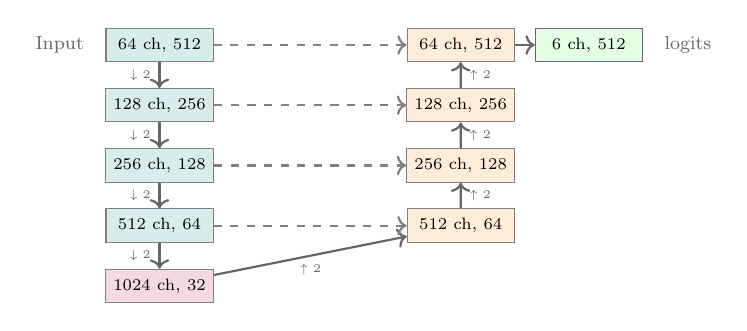
\begin{tikzpicture}[scale=0.85, every node/.style={transform shape}]

  \tikzset{
    enc/.style={draw=black!50, fill=teal!15, minimum width=16mm, minimum height=5mm, font=\scriptsize},
    dec/.style={draw=black!50, fill=orange!15, minimum width=16mm, minimum height=5mm, font=\scriptsize},
    bot/.style={draw=black!50, fill=purple!15, minimum width=16mm, minimum height=5mm, font=\scriptsize},
    skip/.style={->, dashed, thick, black!50},
  }

  % Encoder (top row going down)
  \node[enc] (e1) at (0,0)    {64  ch, 512};
  \node[enc] (e2) at (0,-0.9) {128 ch, 256};
  \node[enc] (e3) at (0,-1.8) {256 ch, 128};
  \node[enc] (e4) at (0,-2.7) {512 ch,  64};
  \node[bot] (bn) at (0,-3.6) {1024 ch, 32};

  % Decoder mirroring on right
  \node[dec] (d4) at (4.5,-2.7) {512 ch,  64};
  \node[dec] (d3) at (4.5,-1.8) {256 ch, 128};
  \node[dec] (d2) at (4.5,-0.9) {128 ch, 256};
  \node[dec] (d1) at (4.5,0)    {64  ch, 512};

  \node[draw=black!60, fill=green!10, minimum width=16mm, minimum height=5mm, font=\scriptsize, right=3mm of d1] (out) {6 ch, 512};

  \node[left=2mm of e1, font=\footnotesize, text=black!60] {Input};
  \node[right=2mm of out, font=\footnotesize, text=black!60] {logits};

  % Down arrows (maxpool)
  \draw[->, thick, black!60] (e1) -- (e2) node[midway, left, font=\tiny] {$\downarrow 2$};
  \draw[->, thick, black!60] (e2) -- (e3) node[midway, left, font=\tiny] {$\downarrow 2$};
  \draw[->, thick, black!60] (e3) -- (e4) node[midway, left, font=\tiny] {$\downarrow 2$};
  \draw[->, thick, black!60] (e4) -- (bn) node[midway, left, font=\tiny] {$\downarrow 2$};

  % Up arrows (transpose conv)
  \draw[->, thick, black!60] (bn) -- (d4) node[midway, below, font=\tiny] {$\uparrow 2$};
  \draw[->, thick, black!60] (d4) -- (d3) node[midway, right, font=\tiny] {$\uparrow 2$};
  \draw[->, thick, black!60] (d3) -- (d2) node[midway, right, font=\tiny] {$\uparrow 2$};
  \draw[->, thick, black!60] (d2) -- (d1) node[midway, right, font=\tiny] {$\uparrow 2$};
  \draw[->, thick, black!60] (d1) -- (out);

  % Skip connections
  \draw[skip] (e1.east) -- (d1.west);
  \draw[skip] (e2.east) -- (d2.west);
  \draw[skip] (e3.east) -- (d3.west);
  \draw[skip] (e4.east) -- (d4.west);

\end{tikzpicture}
\caption{U-Net architecture as implemented. Each rectangle is a \texttt{(Conv3x3
$\rightarrow$ BN $\rightarrow$ ReLU)$\times 2$} block; solid arrows are down/upsampling;
dashed arrows are skip connections concatenated along the channel dimension.}
\label{fig:unet}
\end{figure}

\paragraph{Loss.} Standard pixel-wise cross-entropy over 6 classes:
$
\mathcal{L}_{\text{seg}}(\theta) = -\frac{1}{HW}\sum_{i,j}\sum_{c=0}^{5} y_{ijc}\,\log \hat{y}_{ijc}(\theta).
$

\subsection{YOLOv8 with Oriented Bounding-Box Head}

For the detection branch we use Ultralytics' \texttt{yolov8n-obb.pt} (the ``nano''
variant: $\approx 3$\,M parameters). Compared to the stock YOLOv8 detection head,
the OBB head regresses an additional angle $\theta \in [-\pi/4,\pi/4]$ per anchor
to describe the oriented box, enabling tight enclosures of rotated vehicles that
axis-aligned boxes cannot. Ultralytics handles architecture and loss implementation
internally; the project interacts with it through a thin wrapper in
\texttt{models/yolo.py}.

\paragraph{Why nano.} On an 8\,GB mobile GPU, training YOLOv8-nano at imgsz 1024
is already near the VRAM ceiling once AMP is enabled. The small-, medium-, and
large-variant backbones would require lower batch sizes or smaller input resolutions,
trading detection resolution for backbone capacity. On a two-class dataset
($\approx 9\,000$ labeled vehicles), nano is already more than sufficient.

% =============================================================================
\section{Training Methodology}
% =============================================================================

\subsection{Independent training rationale}

The two models never share gradients. Table~\ref{tab:hparams} highlights how
fundamentally different their training regimes are, reinforcing the decision to
keep them decoupled.

\begin{table}[H]
\centering
\footnotesize
\caption{Training hyperparameters for the two branches.}
\label{tab:hparams}
\begin{tabular}{lll}
\toprule
 & \textbf{U-Net (Potsdam)} & \textbf{YOLOv8-OBB (VSAI)} \\
\midrule
Input size            & $512\times512$                         & $1024\times1024$ \\
Batch size            & 4                                      & 8 \\
Epochs                & 50                                     & 100 (with \texttt{patience=20}) \\
Optimizer             & Adam                                   & SGD + momentum (Ultralytics default) \\
Base LR               & $1\times10^{-4}$                        & $1\times10^{-2}$ (warmup + cosine) \\
Weight decay          & $1\times10^{-5}$                        & $5\times10^{-4}$ \\
LR schedule           & \texttt{ReduceLROnPlateau} (factor 0.5, patience 5) & Cosine anneal + linear warmup \\
Loss                  & Cross-entropy (pixels)                 & DFL + BCE + CIoU/OBB (composite) \\
Augmentations         & HFlip, VFlip, Rot90, Affine, brightness/contrast (Albumentations) & Mosaic, HSV, perspective, mixup (Ultralytics) \\
Mixed precision       & \texttt{torch.amp.autocast("cuda")}    & Automatic (Ultralytics) \\
Evaluation metric     & val cross-entropy + visual mIoU        & mAP$_{50}$ / mAP$_{50:95}$ per class \\
\bottomrule
\end{tabular}
\end{table}

\subsection{Unified configuration}

All hyperparameters live in a single \texttt{config.yaml}. Both training scripts
load this file at startup, so changing training behaviour never requires a code edit.

\begin{lstlisting}[style=yaml, caption={Excerpt of \texttt{config.yaml}.}, label={lst:config}]
device:
  hsa_override_gfx_version: "10.3.0"    # RX 6700S (gfx1032) -> gfx1030 workaround
  num_workers: 4
  amp: true
  seed: 42

unet:
  dataset:
    kagglehub_handle: "deasadiqbal/private-data-1"
    images_subdir: "patches/Images"
    masks_subdir:  "patches/Labels"
  image_size: [512, 512]
  num_classes: 6
  batch_size: 4
  epochs: 50
  lr: 1.0e-4
  train_split: 0.8
  class_info:
    - [0, "impervious_surface", 255, 255, 255]
    - [1, "building",             0,   0, 255]
    # ...

yolo:
  dataset:
    kagglehub_handle: "redzapdos123/vsai-dataset-yolo11-obb-format"
    generated_yaml:   "data/vsai_dataset.yaml"
  model:    "yolov8n-obb.pt"
  imgsz:    1024
  batch:    8
  epochs:   100
  patience: 20
\end{lstlisting}

\subsection{ROCm / HSA override for RX 6700S}

The AMD Radeon RX 6700S uses the \texttt{gfx1032} architecture, which is
\emph{not} on ROCm's officially supported list. However, \texttt{gfx1032} is
binary-compatible with \texttt{gfx1030} (the supported flagship 6900XT). Setting
the environment variable
\[
  \texttt{HSA\_OVERRIDE\_GFX\_VERSION=10.3.0}
\]
before any \texttt{import torch} tricks the HIP runtime into treating the device
as \texttt{gfx1030}, enabling MIOpen kernels to be compiled and loaded.
This override \emph{must} be applied before the first torch import, otherwise
the runtime commits to the wrong target. The project enforces this via
\texttt{utils.device.apply\_hsa\_override()}, which is invoked at the top of
every training and inference entry point:

\begin{lstlisting}[style=python, caption={Top of \texttt{train/train\_unet.py}.}]
from utils.device import apply_hsa_override
apply_hsa_override()   # MUST run before `import torch`

import torch
# ... the rest of the training code
\end{lstlisting}

\subsection{Data augmentation strategy}

U-Net uses Albumentations' image-and-mask-aware transforms so that pixel-level
labels remain consistent through geometric transformations:

\begin{itemize}[leftmargin=*, itemsep=2pt]
  \item \textbf{Train}: \texttt{HorizontalFlip}, \texttt{VerticalFlip},
    \texttt{RandomRotate90}, \texttt{Affine}$(p=0.5)$, \texttt{RandomBrightnessContrast}, ImageNet-style \texttt{Normalize}, \texttt{ToTensorV2}.
  \item \textbf{Val / Inference}: \texttt{Resize} $\rightarrow$ \texttt{Normalize} $\rightarrow$ \texttt{ToTensorV2}.
\end{itemize}

YOLO uses Ultralytics' built-in augmentation pipeline: mosaic (four images
stitched into one to synthesize dense scenes), HSV colour jitter, random perspective,
and mixup.

% =============================================================================
\section{Inference Pipeline}
% =============================================================================

\subsection{Flow}

Figure~\ref{fig:infer} details the inference fusion step. The two models are
applied in sequence; their outputs are expressed in the coordinate system of the
\emph{original} image, and fusion is purely a compositing operation.

\begin{figure}[H]
\centering
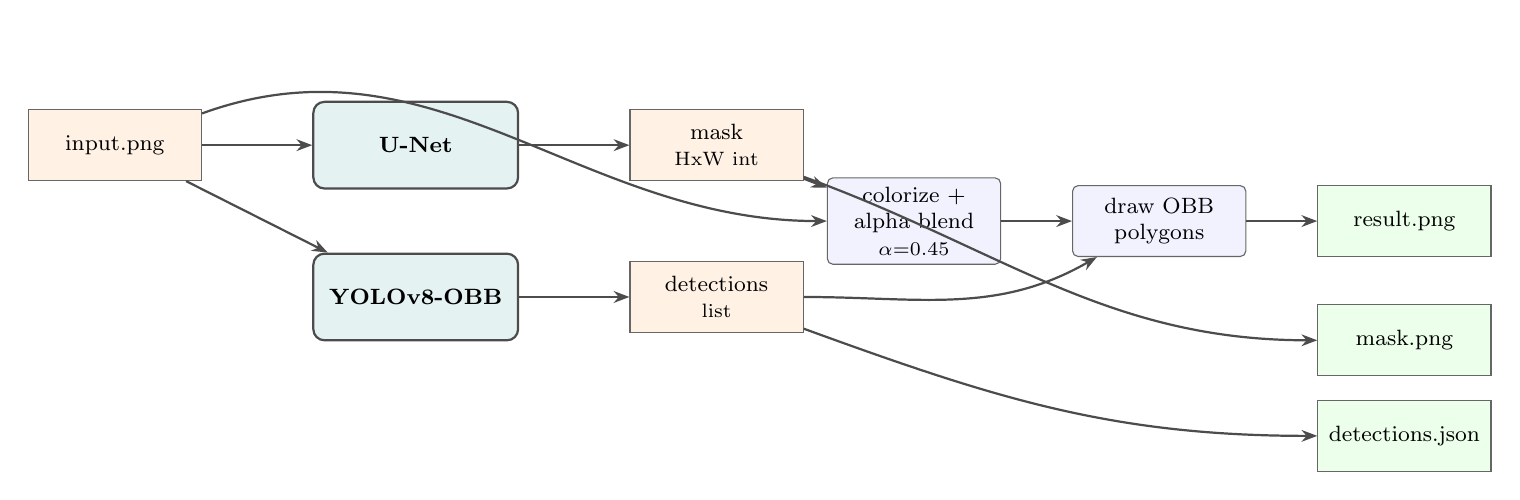
\begin{tikzpicture}[node distance=8mm and 9mm]
  \node[data] (input) {input.png};
  \node[model, right=14mm of input] (unet) {U-Net};
  \node[model, below=of unet] (yolo) {YOLOv8-OBB};
  \node[data, right=14mm of unet]  (mask) {mask\\\scriptsize HxW int};
  \node[data, right=14mm of yolo]  (dets) {detections\\\scriptsize list};
  \node[block, right=14mm of $(mask)!0.5!(dets)$] (overlay) {colorize +\\alpha blend\\\scriptsize $\alpha{=}0.45$};
  \node[block, right=of overlay] (draw)    {draw OBB\\polygons};
  \node[output, right=of draw] (out)       {result.png};

  \draw[arrow] (input) -- (unet);
  \draw[arrow] (input) -- (yolo);
  \draw[arrow] (unet)  -- (mask);
  \draw[arrow] (yolo)  -- (dets);
  \draw[arrow] (mask)  -- (overlay);
  \draw[arrow] (input) to[out=20, in=180] (overlay);
  \draw[arrow] (overlay) -- (draw);
  \draw[arrow] (dets)  to[out=0, in=210] (draw);
  \draw[arrow] (draw)  -- (out);

  \node[output, below=of out, yshift=2mm] (mp) {mask.png};
  \node[output, below=of mp, yshift=5mm]  (dj) {detections.json};
  \draw[arrow] (mask) to[out=-20, in=180] (mp);
  \draw[arrow] (dets) to[out=-20, in=180] (dj);
\end{tikzpicture}
\caption{Inference-time data flow. Three artefacts are written per input image.}
\label{fig:infer}
\end{figure}

\subsection{Fusion details}

The fusion operation is implemented in \texttt{inference/combine.py} and
consists of two steps:

\begin{enumerate}[leftmargin=*]
  \item \textbf{Mask overlay.} The integer class mask is mapped through the
    \texttt{config.yaml} palette to produce a BGR image of identical size,
    then alpha-blended onto the original:
    \[
      C = (1-\alpha)\cdot I + \alpha\cdot M_{\text{color}}, \quad \alpha = 0.45.
    \]
  \item \textbf{OBB polygon draw.} For each detection, the four corner points
    (in original-image pixel coordinates) are connected with \texttt{cv2.polylines}.
    A coloured label box is anchored at the top-left corner with the class name
    and confidence (e.g. \texttt{small-vehicle 0.87}).
\end{enumerate}

\paragraph{What the fusion does \emph{not} do.} It does not use one model's output
to filter or refine the other. There is no cross-model NMS, no mask-gated detection
rejection, no box-guided mask sharpening. This is deliberate: both models are
treated as independent oracles whose outputs are merely co-rendered.

\subsection{Output artefacts}

Three files are written to \texttt{results/inference/}:

\begin{center}\footnotesize
\begin{tabular}{ll}
\toprule
\texttt{result.png}     & composite: original + mask overlay + OBB polygons \\
\texttt{mask.png}       & colorized semantic mask at full resolution (U-Net only) \\
\texttt{detections.json} & list of \{\texttt{class\_id}, \texttt{class\_name}, \texttt{conf}, \texttt{corners}\} \\
\bottomrule
\end{tabular}
\end{center}

% =============================================================================
\section{Engineering Considerations}
% =============================================================================

\subsection{Reproducibility}

\begin{itemize}[leftmargin=*, itemsep=2pt]
  \item Fixed seed (\texttt{config.device.seed = 42}) is set via
    \texttt{torch.manual\_seed}, \texttt{random.seed}, and \texttt{np.random.seed}
    at the start of each training run.
  \item The Potsdam train/val split is deterministic given the seed
    (\texttt{torch.utils.data.random\_split}).
  \item VSAI uses the dataset publisher's fixed split, eliminating
    another source of variance.
  \item Datasets are cached by \texttt{kagglehub} under
    \texttt{\$HOME/.cache/kagglehub/}; repeat runs are free.
\end{itemize}

\subsection{Docker environment}

The \texttt{Dockerfile} builds on \texttt{rocm/pytorch:latest}, which already
contains a ROCm-compatible build of PyTorch, HIP, and MIOpen. Only OS packages
needed by OpenCV (\texttt{libgl1}, \texttt{libglib2.0-0}) and pure-Python
dependencies are added on top. The launcher script \texttt{docker-run.sh} performs:

\begin{lstlisting}[style=bash, caption={Docker launch flags (excerpt).}]
docker run --rm -it \
    --network=host --device=/dev/kfd --device=/dev/dri \
    --ipc=host --shm-size=8G \
    --group-add video \
    -e HSA_OVERRIDE_GFX_VERSION=10.3.0 \
    -e KAGGLE_API_TOKEN="${KAGGLE_API_TOKEN:-}" \
    -v "$PROJECT_DIR":/workspace/aerial -w /workspace/aerial \
    aerial-seg:latest
\end{lstlisting}

The \texttt{--device=/dev/kfd} and \texttt{--device=/dev/dri} flags expose the
GPU to the container; \texttt{--group-add video} grants it access permissions;
\texttt{--ipc=host --shm-size=8G} ensure sufficient shared memory for PyTorch
DataLoader workers.

\subsection{Line-ending and other repo hygiene}

A \texttt{.gitattributes} file enforces LF endings for \texttt{*.sh},
\texttt{Dockerfile}, \texttt{*.py}, and \texttt{*.yaml}. This prevents a common
class of bug on mixed-OS development (e.g., \texttt{env: 'bash\textbackslash r'}
errors when the host uses Windows-style line endings).

% =============================================================================
\section{Testing Strategy}
% =============================================================================

Tests are organized in four layers of increasing cost and scope:

\begin{enumerate}[leftmargin=*, itemsep=4pt]
  \item \textbf{Unit tests (\texttt{tests/test\_*.py}):} pure-Python, no GPU, no
    network. Cover U-Net forward-pass shape correctness, device selection logic,
    config loader round-trips, Potsdam colour-to-class decoding, Albumentations
    train/val contracts, and the OBB polygon drawing primitives.
  \item \textbf{Integration tests:} end-to-end synthetic inference (random
    U-Net $\rightarrow$ random YOLO $\rightarrow$ compose without crashing),
    a 2-batch overfit sanity check on a toy tensor, and VSAI YAML generation
    from a fabricated directory layout.
  \item \textbf{ROCm hardware validation (\texttt{tests/rocm\_check.sh}):} four
    staged checks that run against the real GPU:
    \begin{enumerate}[label=\arabic*.]
      \item \texttt{torch.cuda.is\_available()} and driver/device metadata.
      \item U-Net GPU forward smoke test at batch-2, 512$^2$.
      \item Single optimizer step on the GPU (forward + backward + update).
      \item Optional 1-epoch mini training on each model
        (with \texttt{--with-training} flag).
    \end{enumerate}
  \item \textbf{End-to-end visual check:} run \texttt{infer.py} on a held-out
    image from each dataset and eyeball \texttt{result.png}.
\end{enumerate}

\paragraph{Fast feedback loop.} Layers 1--2 complete in well under a minute and
are run on every code change. Layer 3 takes 1--3 minutes and runs after any
change that touches device, model, or dataset code. Layer 4 runs after training.

% =============================================================================
\section{Experimental Setup and Hardware}
% =============================================================================

\begin{tabular}{ll}
\toprule
GPU                  & AMD Radeon RX 6700S (Navi 23, RDNA2 mobile, \texttt{gfx1032}) \\
VRAM                 & 8\,GB GDDR6 \\
Power budget         & 80--100\,W (dynamic boost) \\
Host OS              & Arch Linux (kernel 6.19) \\
ROCm version (in container) & 7.2 \\
PyTorch              & 2.10.0+rocm7.2.2 \\
HIP version          & 7.2.53211 \\
MIOpen               & bundled with ROCm 7.2 \\
Python               & 3.12 \\
\bottomrule
\end{tabular}

\medskip
\noindent A conservative alternative configuration (\S~\ref{sec:safe}) is used
when thermal or power headroom is constrained.

\subsection{Safe-mode training settings}\label{sec:safe}

For development on the mobile GPU, a conservative configuration keeps sustained
GPU utilization below 85\% while still producing meaningful models:

\begin{center}\footnotesize
\begin{tabular}{lll}
\toprule
                 & \textbf{U-Net}               & \textbf{YOLOv8-OBB} \\
\midrule
Input size       & $320\times320$               & 640 \\
Batch size       & 4                            & 4 \\
Epochs           & 20                           & 30 (\texttt{patience=10}) \\
DataLoader workers & 2                           & 2 \\
Expected wall-clock & $\sim$1.5\,h              & $\sim$15\,min \\
\bottomrule
\end{tabular}
\end{center}

% =============================================================================
\section{Results}
% =============================================================================

The figures below are rendered if the corresponding result files exist in
\texttt{../results/}; otherwise the report compiles with placeholders and the
report author can populate them as training completes.

\subsection{Qualitative inference outputs}

\begin{figure}[H]
\centering
\IfFileExists{../results/inference/result.png}{%
  \includegraphics[width=0.9\linewidth]{../results/inference/result.png}%
}{%
  \fbox{\parbox{0.88\linewidth}{\centering\vspace{6mm}\emph{[Placeholder]}
  \vspace{2mm}\\ Run \texttt{python infer.py --image <path>} to populate
  \texttt{results/inference/result.png}.\vspace{6mm}}}%
}
\caption{Combined inference: U-Net semantic mask alpha-blended over the input,
with YOLOv8 OBB polygons drawn on top.}
\end{figure}

\begin{figure}[H]
\centering
\begin{subfigure}{0.48\linewidth}
  \centering
  \IfFileExists{../results/inference/mask.png}{%
    \includegraphics[width=\linewidth]{../results/inference/mask.png}%
  }{%
    \fbox{\parbox{\linewidth}{\centering\vspace{10mm}\emph{mask.png placeholder}\vspace{10mm}}}%
  }
  \caption{U-Net colourised mask.}
\end{subfigure}\hfill
\begin{subfigure}{0.48\linewidth}
  \centering
  \IfFileExists{../results/yolo/safe/val_batch0_pred.jpg}{%
    \includegraphics[width=\linewidth]{../results/yolo/safe/val_batch0_pred.jpg}%
  }{%
    \fbox{\parbox{\linewidth}{\centering\vspace{10mm}\emph{YOLO predictions placeholder}\vspace{10mm}}}%
  }
  \caption{YOLO OBB predictions on a validation batch.}
\end{subfigure}
\caption{Individual model outputs.}
\end{figure}

\subsection{Training curves (YOLO)}

\begin{figure}[H]
\centering
\IfFileExists{../results/yolo/safe/results.png}{%
  \includegraphics[width=0.95\linewidth]{../results/yolo/safe/results.png}%
}{%
  \fbox{\parbox{0.88\linewidth}{\centering\vspace{6mm}\emph{[Placeholder]}
  \vspace{2mm}\\ Ultralytics writes \texttt{results.png} to
  \texttt{results/yolo/<name>/} after training completes.\vspace{6mm}}}%
}
\caption{YOLOv8-OBB training curves (loss components, mAP$_{50}$,
mAP$_{50:95}$) over epochs.}
\end{figure}

\subsection{Representative metrics (one-epoch smoke test)}

As a sanity check, a single-epoch run on VSAI with \texttt{imgsz=640}, \texttt{batch=2}
produced the following validation metrics, demonstrating that the pipeline is
functional before committing to a full training schedule:

\begin{center}\footnotesize
\begin{tabular}{lrrr}
\toprule
Class & Instances & mAP$_{50}$ & mAP$_{50:95}$ \\
\midrule
small-vehicle & 8\,185 & 0.787 & 0.538 \\
large-vehicle &   288 & 0.102 & 0.066 \\
\textbf{all}   & 8\,473 & \textbf{0.444} & \textbf{0.302} \\
\bottomrule
\end{tabular}
\end{center}

The small-vehicle class already reaches $\mathrm{mAP}_{50}=0.787$ after a single
epoch thanks to the COCO-pretrained backbone. The large-vehicle class is heavily
imbalanced ($\approx 30{:}1$) and would benefit from oversampling or class-weighted loss.

% =============================================================================
\section{Discussion and Limitations}
% =============================================================================

\subsection{Known trade-offs}

\begin{description}[leftmargin=1.2em, style=nextline]
  \item[Cross-domain generalization] U-Net is trained on urban orthophotos (Potsdam)
    and applied at inference to drone-captured scenes (VSAI). Masks on VSAI images
    are therefore noisy; the two datasets cover different domains. A production
    system would either retrain U-Net on a dataset covering the target imagery,
    or train a single model on a dataset carrying both annotation types.
  \item[Fusion is not cross-modal] The two branches do not inform each other's
    predictions. A stronger system would use the mask to filter implausible
    detections (e.g. vehicle centers on \emph{tree} pixels) or use detections to
    refine instance-level mask boundaries.
  \item[Class imbalance in VSAI] Large-vehicle ($N=288$) is 30$\times$ rarer than
    small-vehicle. Even at 100 epochs this class struggles. Mitigations:
    class-balanced sampling, focal loss weighting, or class-specific
    copy-paste augmentation.
  \item[Hardware constraints] On an 80\,W mobile GPU, training is
    thermally bound. Sustained 99\% utilization can push the system into
    thermal throttling. The \S~\ref{sec:safe} ``safe'' configuration trades
    some final accuracy for thermal headroom.
\end{description}

\subsection{What this project demonstrates}

\begin{itemize}[leftmargin=*, itemsep=3pt]
  \item A clean separation between training and inference code, enabling the two
    branches to evolve independently.
  \item End-to-end reproducibility via Docker + \texttt{kagglehub} caching + a
    single \texttt{config.yaml}.
  \item A working ROCm setup on an officially unsupported mobile GPU using
    the \texttt{HSA\_OVERRIDE\_GFX\_VERSION} workaround.
  \item A layered test suite that separates cheap CPU-only checks from expensive
    GPU validation, so iteration stays fast.
\end{itemize}

% =============================================================================
\section{Future Work}
% =============================================================================

\begin{enumerate}[leftmargin=*]
  \item \textbf{Mask-guided NMS.} Reject YOLO detections whose centroid falls
    on \texttt{tree} or \texttt{low\_vegetation} pixels in the U-Net mask.
    20--30 lines in \texttt{inference/pipeline.py}.
  \item \textbf{Per-class mIoU evaluation script.} U-Net currently logs only
    aggregate cross-entropy. A dedicated evaluation routine would compute
    per-class IoU on the held-out split.
  \item \textbf{In-RAM dataset cache.} Potsdam's 2\,400 images decoded to
    numpy ($\approx$2.4\,GB) comfortably fit in RAM; pre-loading would cut
    DataLoader overhead by $\sim$50\%.
  \item \textbf{Joint training experiment.} Train a single encoder with two heads
    (segmentation + detection) on a dataset annotated for both (e.g. iSAID).
    Compare against the current decoupled baseline.
  \item \textbf{Web demo.} A Gradio/Streamlit front-end that accepts an uploaded
    aerial image and displays the fused result.
\end{enumerate}

% =============================================================================
\section*{Appendix A: Quick Start}
\addcontentsline{toc}{section}{Appendix A: Quick Start}
% =============================================================================

\begin{lstlisting}[style=bash, caption={End-to-end reproduction.}]
# 1. Build and launch the Docker container (from repo root on host)
export KAGGLE_API_TOKEN=KGAT_xxxxxxxxxxxxxxxxxxxxx
./docker-run.sh

# 2. Inside the container — validate ROCm
./tests/rocm_check.sh

# 3. Download both datasets (idempotent)
python -m data.download_potsdam
python -m data.download_vsai

# 4. Train (sequential on mobile GPU)
python -m train.train_yolo      # ~15 minutes with patience early-stop
python -m train.train_unet      # ~1.5 - 3 hours depending on config

# 5. Combined inference on any aerial image
python infer.py --image /path/to/image.png
\end{lstlisting}

\begin{thebibliography}{9}
  \bibitem{ronneberger2015unet}
    O.~Ronneberger, P.~Fischer, T.~Brox.
    \emph{U-Net: Convolutional Networks for Biomedical Image Segmentation}.
    MICCAI, 2015.
  \bibitem{yolov8}
    Ultralytics.
    \emph{YOLOv8 Documentation}.
    \url{https://docs.ultralytics.com/}, accessed 2026.
  \bibitem{rocm}
    AMD.
    \emph{ROCm Documentation}.
    \url{https://rocm.docs.amd.com/}, accessed 2026.
  \bibitem{potsdam}
    ISPRS Working Group II/4.
    \emph{2D Semantic Labeling Contest -- Potsdam}.
  \bibitem{vsai}
    Ezzatfar, Ali et al.
    \emph{VSAI: A Multi-view Aerial Imagery Dataset for Vehicle Detection}.
\end{thebibliography}

\end{document}
